\documentclass{article}
\usepackage[left=0.85in, right=0.85in, top=0.5in, bottom=0.95in]{geometry}
\usepackage[T1]{fontenc}
\usepackage[utf8]{inputenc}
\usepackage[italian]{babel}
\usepackage{graphicx}
\usepackage{wrapfig2}
\usepackage{amsmath}
\usepackage{amssymb}
\usepackage{cases}
\usepackage{subcaption}
\usepackage{hyperref}
\hypersetup{
	colorlinks=true,
	linkcolor=blue,    
	urlcolor=blue,
	pdfpagemode=FullScreen,
}
\urlstyle{same}
\usepackage{changepage}
\usepackage{lastpage, epstopdf}
\usepackage{fancyhdr}
\usepackage{tcolorbox}
\usepackage{background}


%=======HEADER & FOOTER=======%
%\def\lesson{Lesson Title}
%\def\outcome{\textbf{Learning Outcomes:} Outcomes go here. }

%\pagestyle{fancy}
%\fancyhf{}
%\renewcommand{\headrulewidth}{0pt}
%\renewcommand{\footrulewidth}{1.4pt}
%\lfoot{My Name $\diamond$ \the\year}
%\cfoot{Page \thepage/\pageref{LastPage}}
%\rfoot{\lesson}

%=======CORNELL STYLE FORMAT=======%
\SetBgScale{1}
\SetBgAngle{0}
\SetBgColor{black}
\SetBgContents{\rule{1pt}{0.899\paperheight}}
\SetBgHshift{-1.6in}
\SetBgVshift{-0.1in}

%=======CUSTOM BOXES=======%

\parindent 0ex

%=======BODY=======%
\begin{document}
%	\setcounterpageref{secnumdepth}{0}
	\section*{MECCANICA DEI SOLIDI: PARTE 2} %Date: \hrulefill}
%	\begin{tcolorbox}{\outcome}\end{tcolorbox}
	
	\begin{adjustwidth}{2in}{} 
		
	{\Large \textbf{Vincoli interni nel piano}} \mbox{} \newline
		I vincoli che agiscono tra un corpo e un riferimento assoluto solidale a terra, sono detti vincoli esterni. 
		
		Quando un vincolo agisce sullo spostamento relativo, ovvero sullo spostamento di un corpo rispetto ad un sistema di riferimento solenoidale ad un altro, è detto vincolo interno. \newline
		
		\textbf{Spostamenti relativi} \newline
		Dati due corpi rigidi, per ciascuno di essi si può definire un campo di spostamenti virtuali. 
		
		Si immagini i corpi rispettivamente appartenenti a due piani mobili cosicché P ed O appartengano ai rispettivi piani, con le relazioni che seguono si possono scrivere gli spostamenti di un qualsiasi punto pensato solidale al corpo.

		
		\[\begin{split}
			\vec{s_P}' & = \vec{s_O}' + \vec{\Phi}' \times (P-O) \\
			\vec{s_P}'' & = \vec{s_O}'' + \vec{\Phi}'' \times (P-O)
		\end{split}
		\]
		È bene notare che O e P NON appartengono ai corpi specifici, ma giacciono sul piano mobile infinitamente esteso e solidale al campo in esame.
		
		Si definisce quindi lo spostamento relativo del corpo $II$ rispetto al corpo $I$:
		\[
		\vec{s_P}^{'', '} = \vec{s_P}'' - \vec{s_P}' = \vec{s_O}'' - \vec{s_O}'  + (\vec{\Phi}'' - \vec{\Phi}') \times (P-O) = \vec{s_O}^{'', '} + \vec{\Phi}^{'', '} \times (P-O)
		\]
		I vincoli interni sono situati tra due corpi e ne limitano lo spostamento relativo. Un vincolo interno lo si pone sempre essere un vincolo puntiforme condiviso tra due corpi. \newline
		
		\begin{enumerate}
			\item \textbf{Cerniera Interna} \newline
			\begin{figure}[H]
				\centering
				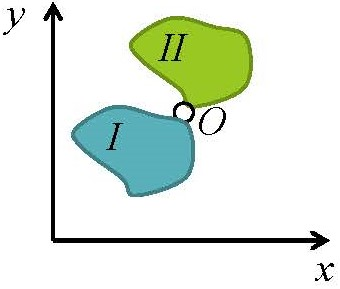
\includegraphics[width=0.25\linewidth]{immagini/1.PARTE2_Pagina_03}
			\end{figure}
			Sono impedite tutte le traslazioni relative, mentre non si oppone alle rotazioni relative.
			
			Possono spostarsi I e II? Si, ma della stessa quantità
			\[
			\vec{s_O}^{'', '} = 0 \Rightarrow \vec{s_O}'' - \vec{s_O}' = 0 \Rightarrow \begin{cases}
				\vec{s_O}'' - \vec{s_O}' = 0 \\
				\vec{M_O} = 0
			\end{cases}
		\]
		\[
		\left[\begin{array}{cccccc}
			1 & 0 & 0 & -1 & 0 & 0 \\
			0 & 1 & 0 & 0 & -1 & 0
		\end{array} \right] \left[ \begin{array}{c}
		s'_{Ox} \\
		s'_{Oy} \\
		\varphi'_z \\
		s''_{Ox} \\
		s''_{Oy} \\
		\varphi''_z
	\end{array}\right] = \left\lbrace 0 \right\rbrace
		\]
			\[
			\begin{cases}
				s'_{Ox} = s''_{Ox} \\
				s'_{Oy} = s''_{Oy}
			\end{cases} \Rightarrow MC = 2
			\]
			
			Per ottenere le equazioni statiche impongo il vincolo liscio: 
			\[
			L_{V} = 0 ~ \forall ~ \vec{s_P} = 0 : \vec{s_O}^{'', '} = 0
			\]
			E allora:
			\[
				L_{V} = \vec{R}' \cdot \vec{s_O}'+ \vec{\Phi}' \cdot \vec{M_O}'+ \vec{R}'' \cdot \vec{s_O}''+ \vec{\Phi}'' \cdot \vec{M_O}'' = 0
			\]
			Applicando gli spostamenti compatibili $ \vec{s_O}'' = \vec{s_O}' = 0 $ si ottiene:
			\[
				L_{V} = \vec{\Phi}' \cdot \vec{M_O}'+ \vec{\Phi}'' \cdot \vec{M_O}'' = 0
			\]
			Imponendo $ \vec{\Phi}' = 0 $ ottengo $ L_{V} = \vec{\Phi}'' \cdot \vec{M_O}'' = 0 \Rightarrow \vec{M_O}'' = 0 $.
			
			Si può riscrivere a questo punto il lavoro virtuale come:
			\[
			L_{V} = \vec{\Phi}' \cdot \vec{M_O}' = 0
			\]
			Imponendo di nuovo gli spostamento compatibili ottengo:  \[L_{V} = \vec{\Phi}' \cdot \vec{M_O}' = 0 \Rightarrow \vec{M_O}' = 0 \]
			
			Il lavoro virtuale di una cerniera è dunque, ricordando che $\vec{s_O}' = \vec{s_O}''$: 
			\[
			L_{V} = \vec{R}' \cdot \vec{s_O}'+ + \vec{R}'' \cdot \vec{s_O}'' = 0 \Rightarrow (\vec{R}' + \vec{R}'') \cdot \vec{s_O}'' = 0 \Rightarrow \vec{R}' = - \vec{R}''
			\]
			In pieno accordo al principio di azione e reazione. 
			
			Infine 
			\[
			\left\lbrace R_1 = (\lambda_1 \hat{i} + \lambda_2 \hat{j}; 0); R_2 = (-\lambda_1 \hat{i} - \lambda_2 \hat{j}; 0); M=0\right\rbrace 
			\]
			Dovendo imporre due reazioni vincolari $\lambda_1, \lambda_2$, la molteplicità statica sarà $MS = 2$. \newpage
			
			\item \textbf{Pendolo Interno} \newline
				\begin{figure}[H]
				\centering
				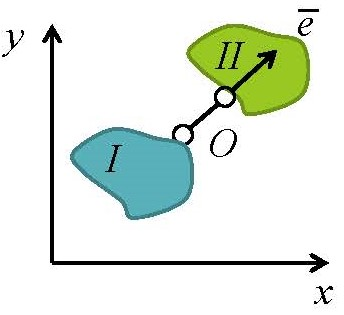
\includegraphics[width=0.25\linewidth]{immagini/1.PARTE2_Pagina_06}
			\end{figure}
			Sono impedite le traslazioni relative in direzione $\vec{e}$ asse del pendolo, mentre sono libere quelle ortogonali ad $\vec{e}$, sono libere anche le rotazioni relative: tra di loro i corpi non si possono allontanare in direzione dell'asse del pendolo ma possono solo avere spostamenti relativi perpendicolari a tale asse.
			\[
			(1)~\vec{s_O}'' \cdot \vec{e} - \vec{s_O}' \cdot \vec{e} = 0 \Rightarrow \vec{s_O}'' \cdot \vec{e} = \vec{s_O}' \cdot \vec{e} 
			\]
			\[
			\left[ \begin{array}{cccccc}
				e_x & e_y & 0  & -e_x & -e_y & 0
			\end{array}\right] \left[ \begin{array}{c}
			s'_{0x} \\
			s'_{0y} \\
			\varphi'_z \\
			s''_{0x} \\
			s''_{0y} \\
			\varphi''_z
		\end{array}\right] = \left\lbrace 0 \right\rbrace \Rightarrow MC = 1
			\]
			Le reazioni vincolari saranno quelle duali agli spostamenti vincolati:
				\[
			L_{V} = \vec{R}' \cdot \vec{s_O}'+ \vec{\Phi}' \cdot \vec{M_O}'+ \vec{R}'' \cdot \vec{s_O}''+ \vec{\Phi}'' \cdot \vec{M_O}'' = 0
			\]
			Tra tutti, si sceglie di valutare questi possibili spostamenti compatibili: $ \vec{s_O}' = \vec{s_O}'' = \vec{\Phi}' = 0$
				\[
			L_{V} =  \vec{\Phi}'' \cdot \vec{M_O}'' \underset{\forall\varphi}{=} 0 \Rightarrow  \vec{M_O}'' = 0
			\]
			Allora: 
				\[
			L_{V} = \vec{R}' \cdot \vec{s_O}'+ \vec{\Phi}' \cdot \vec{M_O}'+ \vec{R}'' \cdot \vec{s_O}'' = 0
			\]
			Si scelgono altri possibili spostamenti compatibili: $ \vec{s_O}' = \vec{s_O}''= 0$
			\[
			L_{V} =  \vec{\Phi}' \cdot \vec{M_O}' = 0 \Rightarrow  \vec{M_O}' = 0
			\]	
			Noto ciò, si ottiene che il lavoro virtuale per un pendolo interno è: 
				\[
		(2)~L_{V} = \vec{R}' \cdot \vec{s_O}'+ \vec{R}'' \cdot \vec{s_O}'' = 0
			\]	
			Se si avesse lo spostamento $\vec{s_O}'' = 0$:
				\[
			L_{V} = \vec{R}' \cdot \vec{s_O}' = 0 \Rightarrow \begin{cases}
\vec{R}' \perp \vec{s_O}'\\
\vec{s_O}' \perp \vec{e} 
			\end{cases} \Rightarrow  \vec{R}' \parallel \vec{e}
			\]	
			Oppure se si avesse lo spostamento $\vec{s_O}' = 0$:
			\[
			L_{V} = \vec{R}'' \cdot \vec{s_O}'' = 0 \Rightarrow \begin{cases}
				\vec{R}'' \perp \vec{s_O}''\\
				\vec{s_O}'' \perp \vec{e} 
			\end{cases} \Rightarrow  \vec{R}'' \parallel \vec{e}
			\]	
			Perciò:
			\[
			\begin{cases}
(1)~\vec{s_O}'' \cdot \vec{e} = \vec{s_O}' \cdot \vec{e} \\
(2)~\vec{R}' \cdot \vec{s_O}' + \vec{R}'' \cdot \vec{s_O}'' = 0
			\end{cases} \Rightarrow \vec{R}' \cdot \vec{s_O}' = - \vec{R}'' \cdot \vec{s_O}'' \Rightarrow  \vec{R}' = -\vec{R}''
			\]
			\[
			\begin{cases}
				\vec{R}' = (\lambda_1 \vec{e}; 0) \\
				\vec{R}'' = (-\lambda_1 \vec{e}; 0) \\
				\vec{M_O}'= \vec{M_O}'' = 0
			\end{cases}
			\]
Con una sola reazione vincolare $\lambda_1$ da imporre, $MS = 1$. \newline

\item \textbf{Incastro Interno} \newline
	\begin{figure}[H]
	\centering
	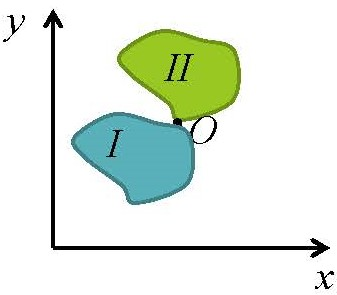
\includegraphics[width=0.25\linewidth]{immagini/1.PARTE2_Pagina_09}
\end{figure}
Sono impedite tutte le traslazioni e le rotazione relative.
\[
\begin{cases}
\vec{s_O}^{'', '} = 0 \\
\vec{\Phi}^{'', '} = 0
\end{cases} \Rightarrow \begin{cases}
\vec{s_O}' = \vec{s_O}'' \\
\vec{\Phi}' = \vec{\Phi}''
\end{cases} \Rightarrow \begin{cases}
s'_{0x} = s''_{0x} \\
s'_{0y} = s''_{0y} \\
\varphi'_z = \varphi''_z \\
\end{cases}
\]
\[
\left[ \begin{array}{cccccc}
	1 & 0 & 0 & -1 & 0 & 0 \\
	0 & 1 & 0 & 0 & -1 & 0 \\
	0 & 0 & 1 & 0 & 0 & -1
\end{array}\right] \left[ \begin{array}{c}
s'_{0x} \\
s'_{0y} \\
\varphi'_z \\
s''_{0x} \\
s''_{0y} \\
\varphi''_z
\end{array}\right] = \left\lbrace 0 \right\rbrace \Rightarrow MC = 3
\]
Il vincolo inibisce qualsiasi rotazione e traslazione, reagirà con un momento qualunque ed una forza qualsiasi.

Per il principio di azione e reazione varrà:
\[
\vec{R}' = -\vec{R}''; \vec{M_O}' = -\vec{M_O}''
\]
\[
L_V = \vec{R}' \cdot \vec{s_O}'+ \vec{\Phi}' \cdot \vec{M_O}'+ \vec{R}'' \cdot \vec{s_O}''+ \vec{\Phi}'' \cdot \vec{M_O}'' = 0 
\]
I possibili spostamenti compatibili sono: 
\[
\vec{s_O}'' = \vec{s_O}' = \vec{\Phi}' = \vec{\Phi}'' = 0
\]
è dunque verificata la condizione per cui, per un vincolo liscio, si deve avere:
\[
L_V = 0
\]
Pertanto $ \forall ~ \vec{R}', \vec{R}''; \vec{M_O}', \vec{M_O}''$ varrà:
\[
\begin{cases}
\vec{R}' = (\lambda_1 \hat{i} + \lambda_2 \hat{j}; 0) \\
\vec{R}'' = (-\lambda_1 \hat{i} - \lambda_2 \hat{j}; 0)\\
\vec{M_O}' = (\lambda_3\hat{k}; 0) \\
\vec{M_O}'' = (-\lambda_3\hat{k}; 0)
\end{cases}
\]				
Dovendo imporre 3 reazioni vincolari $\lambda_1, \lambda_2, \lambda_3$ si avrà $MS = 3$. \newline	
\newpage			
\item \textbf{Doppio Pendolo Interno} \newline	
	\begin{figure}[H]
	\centering
	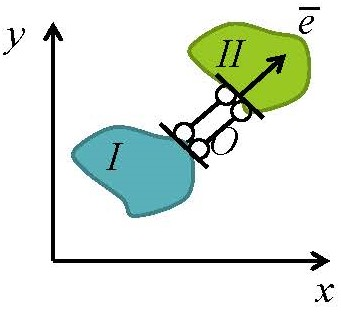
\includegraphics[width=0.25\linewidth]{immagini/1.PARTE2_Pagina_11}
\end{figure}			
Sono impedite le rotazioni relative e le traslazioni relative in direzione di $\vec{e}$.
\[
\begin{cases}
	\vec{s_O}^{'', '} \cdot \vec{e} = 0 \\
	\vec{\Phi}^{'', '} = 0
\end{cases} \Rightarrow \begin{cases}
	\vec{s_O}' \cdot \vec{e} = \vec{s_O}'' \cdot \vec{e} \\
	\vec{\Phi}' = \vec{\Phi}''
\end{cases} \Rightarrow MC = 2
\]				
\[
\left[ \begin{array}{cccccc}
	e_x & e_y & 0 & -e_x & -e_y & 0 \\
	0 & 0 & 1 & 0 & 0 & -1 	
\end{array}\right] \left[ \begin{array}{c}
	s'_{0x} \\
	s'_{0y} \\
	\varphi'_z \\
	s''_{0x} \\
	s''_{0y} \\
	\varphi''_z
\end{array}\right] = \left\lbrace 0 \right\rbrace
\]
Le reazioni vincolari saranno quelle duali agli spostamenti vincolati:
\[
L_{V} = \vec{R}' \cdot \vec{s_O}'+ \vec{\Phi}' \cdot \vec{M_O}'+ \vec{R}'' \cdot \vec{s_O}''+ \vec{\Phi}'' \cdot \vec{M_O}'' = 0
\]
Se scelgo come possibili spostamenti compatibili: $ \vec{s_O}' = \vec{s_O}'' = 0$
\[ 
L_{V} =  \vec{\Phi}' \cdot \vec{M_O}'+ \vec{\Phi}'' \cdot \vec{M_O}'' = 0
\]
Se scelgo come possibili rotazioni compatibili: $ \vec{\Phi}' = \vec{\Phi}'' = \vec{\Phi}$
\[
L_{V} =  \vec{\Phi} \cdot (\vec{M_O}' + \vec{M_O}'') = 0 \Rightarrow \vec{M_O}' = - \vec{M_O}''
\]
Se scelgo come possibili rotazioni compatibili: $ \vec{\Phi}' = \vec{\Phi}'' = \vec{\Phi} = 0$
\[
L_{V} = \vec{R}' \cdot \vec{s_O}'+ \vec{R}'' \cdot \vec{s_O}'' = 0
\]

Se si avesse $\vec{s_O}'' = 0$:
	\[
L_{V} = \vec{R}' \cdot \vec{s_O}' = 0 \Rightarrow \begin{cases}
	\vec{R}' \perp \vec{s_O}'\\
	\vec{s_O}' \perp \vec{e} 
\end{cases} \Rightarrow  \vec{R}' \parallel \vec{e}
\]	
Oppure se si avesse  $\vec{s_O}' = 0$:
\[
L_{V} = \vec{R}'' \cdot \vec{s_O}'' = 0 \Rightarrow \begin{cases}
	\vec{R}'' \perp \vec{s_O}''\\
	\vec{s_O}'' \perp \vec{e} 
\end{cases} \Rightarrow  \vec{R}'' \parallel \vec{e}
\]	
Perciò:
\[
\begin{cases}
	\vec{s_O}'' \cdot \vec{e} = \vec{s_O}' \cdot \vec{e} \\
	\vec{R}' \cdot \vec{s_O}' + \vec{R}'' \cdot \vec{s_O}'' = 0
\end{cases} \Rightarrow \vec{R}' \cdot \vec{s_O}' = - \vec{R}'' \cdot \vec{s_O}'' \Rightarrow  \vec{R}' = -\vec{R}''
\]
\[
\begin{cases}
	\vec{R}' = (\lambda_1 \vec{e}; 0) \\
	\vec{R}'' = (-\lambda_1 \vec{e}; 0) \\
	\vec{M_O}'= (\lambda_2 \hat{k}; 0) \\
	\vec{M_O}'' = (-\lambda_2 \hat{k}; 0)
\end{cases}
\]
Con due sole reazioni vincolari $\lambda_1, \lambda_2$ da imporre, $MS = 2$. \newline

\item \textbf{Doppio Doppio Pendolo Interno} \newline	
	\begin{figure}[H]
	\centering
	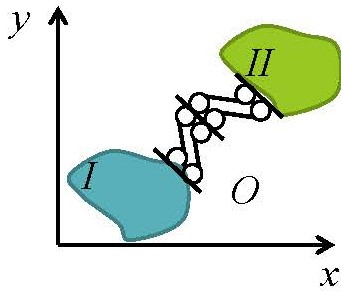
\includegraphics[width=0.25\linewidth]{immagini/1.PARTE2_Pagina_14}
\end{figure}
Sono impedite le rotazioni relative.
\[
\vec{\Phi}^{'', '} = 0 \Rightarrow \vec{\Phi}'= \vec{\Phi} \Rightarrow MC =1 
\]
\[
\left[ \begin{array}{cccccc}
	0 & 0 & 1 & 0 & 0 & -1 
		
\end{array}\right] \left[ \begin{array}{c}
	s'_{0x} \\
	s'_{0y} \\
	\varphi'_z \\
	s''_{0x} \\
	s''_{0y} \\
	\varphi''_z
\end{array}\right] = \left\lbrace 0 \right\rbrace
\]
Opponendosi alla rotazione genera un momento, mentre lasciando libere le traslazioni non genera forze vincolari. 
Possibili spostamenti compatibili: $ \vec{s_O}' = \vec{s_O}'' = 0$
\[ 
L_{V} =  \vec{\Phi}' \cdot \vec{M_O}'+ \vec{\Phi}'' \cdot \vec{M_O}'' = 0
\]
Possibili spostamenti compatibili: $ \vec{\Phi}' = \vec{\Phi}'' = \vec{\Phi}$
\[
L_{V} =  \vec{\Phi} \cdot (\vec{M_O}' + \vec{M_O}'') = 0 \Rightarrow \vec{M_O}' = - \vec{M_O}''
\]
Affinché le rotazioni siano tra loro uguali.

Possibili spostamenti compatibili: $ \forall ~\vec{s_O}$


Se si avesse $\vec{s_O}'' = 0$:
\[
L_{V} = \vec{R}' \cdot \vec{s_O}' = 0 \Rightarrow \vec{R}' = 0 \forall ~\vec{s_O}'
\]	
Oppure se si avesse  $\vec{s_O}' = 0$:
\[
L_{V} = \vec{R}'' \cdot \vec{s_O}'' = 0 \Rightarrow \vec{R}'' = 0 \forall ~\vec{s_O}''
\]	
Perciò:
\[
\begin{cases}
	\vec{R}' = 0 \\
	\vec{R}'' = 0 \\
	\vec{M_O}'= (\lambda_1 \hat{k}; 0) \\
	\vec{M_O}'' = (-\lambda_1 \hat{k}; 0)
\end{cases}
\]
Con una sola reazione vincolare $\lambda_1$ da imporre, $MS = 1$.		
		\end{enumerate} 
	\newpage
Esempio: tante reazioni vincolari quanti corpi.\newline
Cosa succede se ad un vincolo interno vengono collegati più di due corpi? Aumentano le equazioni di vincolo.
	\begin{figure}[H]
	\centering
	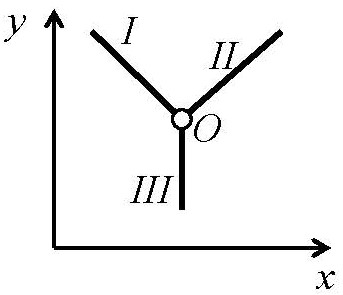
\includegraphics[width=0.25\linewidth]{immagini/1.PARTE2_Pagina_16}
\end{figure}
Cerniera
\[ 
\begin{cases}
\vec{s_O}^{'', '} = 0 \\
\vec{s_O}^{''', '} = 0 \\
\vec{s_O}^{''', ''} = 0
\end{cases} \Rightarrow \begin{cases}
\vec{s_O}'' = \vec{s_O}' \\
\vec{s_O}''' = \vec{s_O}' \\
\vec{s_O}''' = \vec{s_O}''
\end{cases}
\]
 È $MC=6$? Se lo spostamento di I dev'essere uguale allo spostamento di II e lo spostamento di II dev'essere uguale allo spostamento di III , serve dire che lo spostamento di II è uguale allo spostamento di III? No, è combinazione lineare, la molteplicità cinematica è uguale a 4!
 
 La cerniera non si oppone alla rotazione, per cui: $\vec{M_O}' = \vec{M_O}'' = \vec{M_O}''' = 0$ 
 
 Per l'equilibrio: $ \vec{R}' + \vec{R}'' + \vec{R}''' = 0 \Rightarrow \vec{R}' + \vec{R}'' = - \vec{R}''$ 
 
 E dunque: 
 
\[
\begin{cases}
\vec{R}' = (\lambda_1 \hat{i} + \lambda_2 \hat{j}; 0) \\
\vec{R}'' = (\lambda_3 \hat{i} + \lambda_4 \hat{j}; 0) \\
\vec{R}''' = [-(\lambda_1 - \lambda_3) \hat{i} - (\lambda_2 - \lambda_4) \hat{j}; 0] \\
\vec{M_O}' = \vec{M_O}'' = \vec{M_O}'''
\end{cases}
\]
\newpage
Esempio: \newline
	\begin{figure}[H]
	\centering
	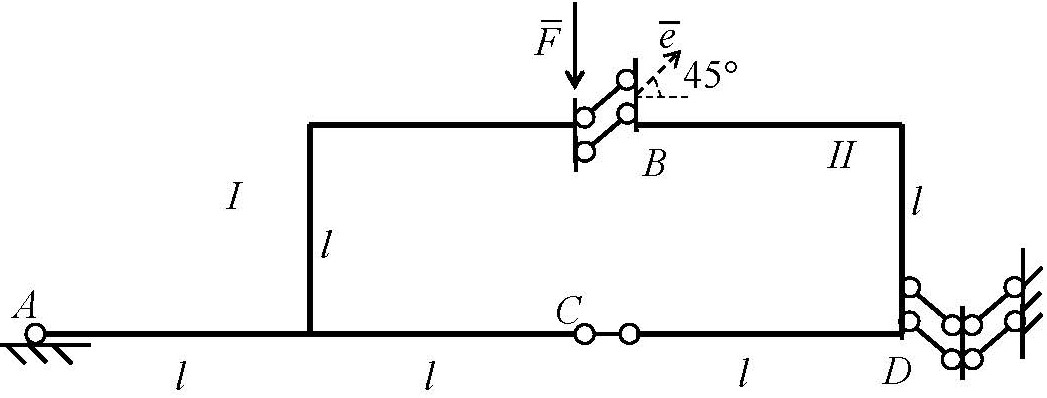
\includegraphics[width=0.4\linewidth]{immagini/1.PARTE2_Pagina_17 (2)}
\end{figure}
\begin{itemize}
\item A: Cerniera esterna $\rightarrow MC=2$;
\item B: D. Pendolo interno $\rightarrow MC=2$;
\item C: Pendolo interno $\rightarrow MC=1$;
\item D: D. D. Pendolo esterno $\rightarrow MC=1$;
\end{itemize}

Ottenendo un numero di vincoli semplici pari a $ s = 6$, ho dunque bisogno di 6 reazioni vincolari $\lambda$ per risolvere l'equilibrio.
\begin{figure}[H]
	\centering
	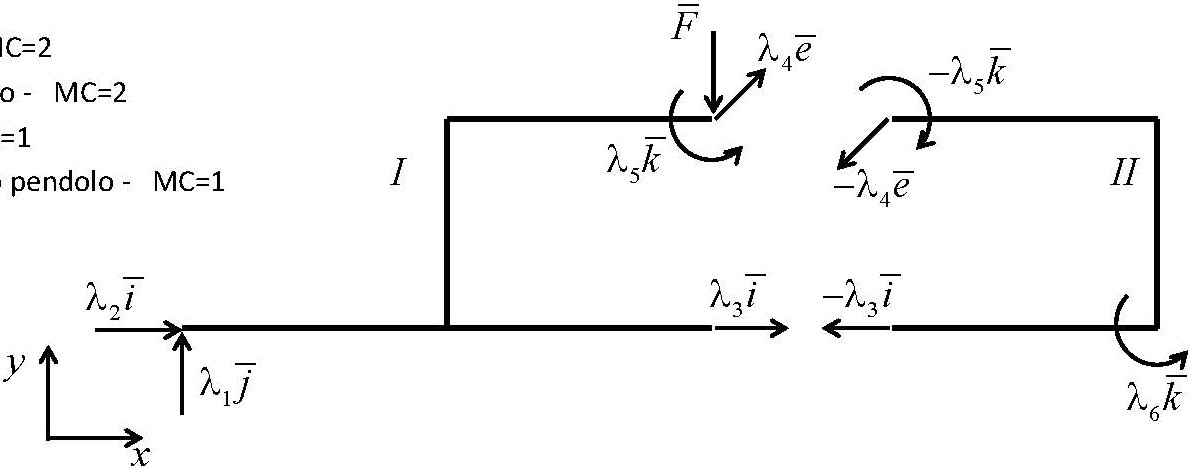
\includegraphics[width=0.4\linewidth]{immagini/1.PARTE2_Pagina_17}
\end{figure}

\textbf{NB}: Per i momenti, con un'asse z uscente dal foglio, il segno positivo è antiorario. \newline

Per il corpo 1: 
\[
\vec{R}' = \lambda_2 \hat{i} + \lambda_1 \hat{j} + \lambda_3 \hat{i} + \lambda_4 \cdot \vec{e} - F \hat{j} = 0
\]

\[
\vec{M_A}' = \text{tutte le forze} \times \text{tutti i bracci} + \text{momenti concentrati}
\]
\begin{enumerate}
\item 
\[
\begin{split}
\vec{M_1} & =(B-A) \times \lambda_4\cdot\vec{e} \\
& = (2l\hat{i} + l\hat{j}) \times \lambda_4\cdot\vec{e} = \\
& = 2l\hat{i} \times \left[ \lambda_4\left(  \frac{\sqrt{2}}{2}\hat{i} + \frac{\sqrt{2}}{2}\hat{j} \right)  \right]  + l\hat{j} \times \left[ \lambda_4\left(  \frac{\sqrt{2}}{2}\hat{i} + \frac{\sqrt{2}}{2}\hat{j} \right) \right]  \\
& = 2l\lambda_4 \frac{\sqrt{2}}{2} \hat{k} + \left( -l\lambda_4 \frac{\sqrt{2}}{2} \hat{k}\right)  
\end{split}
\]
\item 
\[
\vec{M_2}  = (B-A) \times -(F\hat{j})= 2l\hat{i} \times -F\hat{j} = -2lF\hat{k}
\]
\item 
\[
\vec{M_3}  = \lambda_5 \hat{k}
\]
\end{enumerate} 
Infine:
\[
\vec{M_A}' = 2l\lambda_4 \frac{\sqrt{2}}{2} \hat{k} + \left( -l\lambda_4 \frac{\sqrt{2}}{2} \hat{k}\right) -2lF\hat{k} + \lambda_5 \hat{k}
\]
Reminder: Il momento di $\lambda_3$ è nullo per il primo corpo e questo lo si scopre, o semplicemente calcolandolo $2l\hat{i} \times \lambda_3\hat{i} = 0$, oppure accorgendosi che $\lambda_3$ passa esattamente per il polo A e dunque ha braccio nullo. \newline

Per il corpo 2:
\[
\vec{R}'' = -\lambda_3 \hat{i} - \lambda_4 \cdot \vec{e}  = 0
\]
\[
\vec{M_B}'' = \text{tutte le forze} \times \text{tutti i bracci} + \text{momenti concentrati}
\]
\begin{enumerate}
	\item 
	\[
	\vec{M_1} = -\lambda_5 \hat{k} 
	\]
	\item 
	\[
	\vec{M_2} = \lambda_6 \hat{k}
	\]
	\item 
	\[
	\vec{M_3} = (C-B)\times -\lambda_3 \hat{i} = -l\hat{j} \times -\lambda_3 \hat{i} = -l\lambda_3\hat{k}
	\]
\end{enumerate}

\[
\vec{M_B}'' = -l\lambda_3\hat{k} -\lambda_5 \hat{k}  + \lambda_6 \hat{k}
\]
		
Allora, per componenti: 
\[
\begin{cases}
	R_{1x} = \lambda_2 + \lambda_3 + \lambda_4\frac{\sqrt{2}}{2} = 0 \\
	R_{1y} = \lambda_1 + \lambda_4\frac{\sqrt{2}}{2} - F = 0 \\
	M_{1Az} = l\lambda_4\frac{\sqrt{2}}{2} - 2lF + \lambda_5 \\
	
	R_{2x} = -\lambda_3 - \lambda_4\frac{\sqrt{2}}{2} = 0 \\
	R_{2y} = - \lambda_4\frac{\sqrt{2}}{2}  = 0 \\
	M_{2Bz} = +\lambda_6 -l\lambda_3 - \lambda_5 \\
	\end{cases}
\]	
In forma matriciale:
\[
\left[ \begin{array}{cccccc}
	0 & 1 & 1 & \frac{\sqrt{2}}{2} & 0 & 0 \\
	1 & 0 & 0 & \frac{\sqrt{2}}{2} & 0 & 0 \\
	0 & 0 & 0 & l\frac{\sqrt{2}}{2} & 1 & 0 \\
	0 & 0 & -1 & -\frac{\sqrt{2}}{2} & 0 & 0 \\
	0 & 0 & 0 & -\frac{\sqrt{2}}{2} & 0 & 0 \\
	0 & 0 & -l & 0 & -1 & 1
\end{array}\right] \left[ \begin{array}{c}
\lambda_1 \\
\lambda_2\\
\lambda_3\\
\lambda_4\\
\lambda_5\\
\lambda_6
\end{array}\right] = \left[ \begin{array}{c}
0 \\
F \\
2lF \\
0 \\
0 \\
0
\end{array}\right] 
\]
Applicando il Metodo di Gauss alla matrice completa del sistema (unico e solo modo per applicarlo, ricordati che va portato dietro anche il termine noto), si perviene a: 
\[
\begin{array}{c}

[E] = \left[\begin{array}{ccccccc}
	1 & 0 & 0 & \frac{\sqrt{2}}{2} & 0 & 0 & -F \\
	0 & 1 & 1 & \frac{\sqrt{2}}{2} & 0 & 0 & 0 \\
	0 & 0 & -1 & -\frac{\sqrt{2}}{2} & 0 & 0 & 0 \\
	0 & 0 & 0 & -\frac{\sqrt{2}}{2} & 0 & 0 & 0 \\
	0 & 0 & 0 & 0 & 2 & -1 & -2lF \\
	0 & 0 & 0 & 0 & 0 & 1/2 & -2lF
\end{array} \right] \Rightarrow rk(E) = 6 \Rightarrow  ~ \exists! ~  S: \\
S = \begin{cases}
	\lambda_1 = F \\
	\lambda_2 = \lambda_3 = \lambda_4 = 0\\
	\lambda_5 = \lambda_6 = 2Fl
	\end{cases}
\end{array}
\]
\begin{figure}[H]
	\centering
	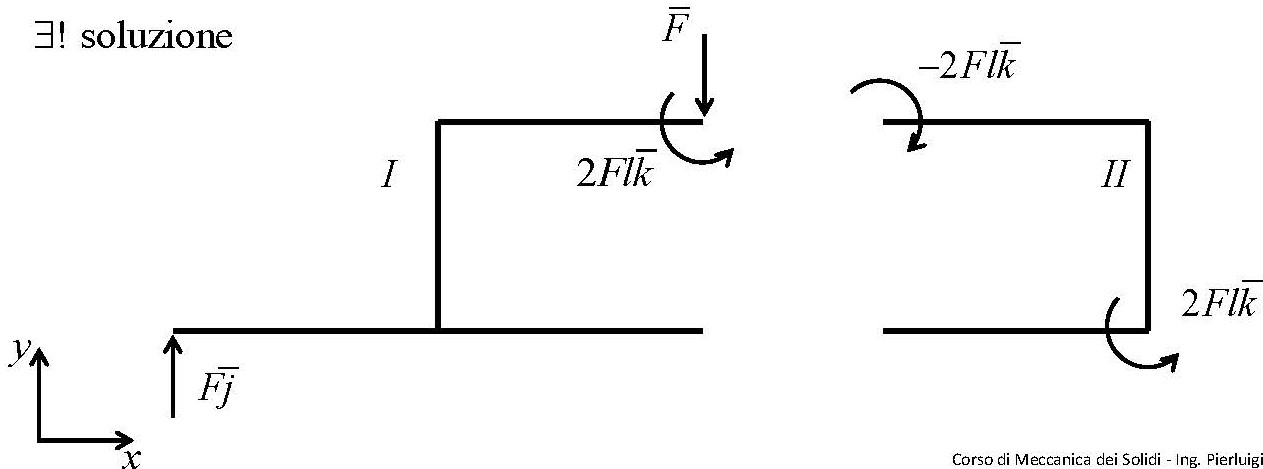
\includegraphics[width=0.4\linewidth]{immagini/1.PARTE2_Pagina_20}
\end{figure}
\newpage
	{\Large \textbf{Carichi distribuiti}} \mbox{} \newline
	Poiché nella realtà non si avranno mai forze concentrate ma sempre una distribuzione di queste, si introducono le forze distribuite ogni qualvolta il carico non sia più concentrato in un punto di applicazione ma ogni elemento infinitesimo di struttura risulti caricato. 
	
	Classico esempio è il carico proprio della struttura. \newline
	
	Definisco "z" ascissa curvilinea.\newline 
	
	\textbf{Forza Distribuita}		
		
		\begin{figure}[H]
			\centering
			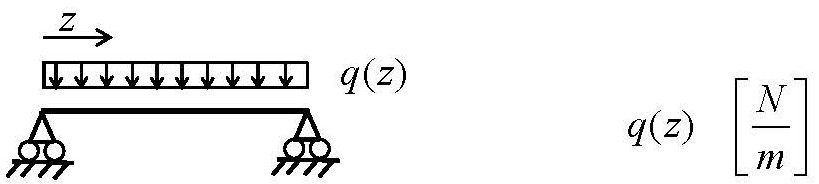
\includegraphics[width=0.4\linewidth]{immagini/1.PARTE2_Pagina_21 (2)}
		\end{figure}
		
	\textbf{Momento Distribuito}	
	
		\begin{figure}[H]
			\centering
			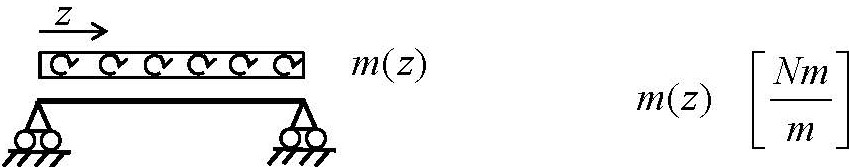
\includegraphics[width=0.4\linewidth]{immagini/1.PARTE2_Pagina_21}
		\end{figure}
	
	Il carico in direzione assiale viene chiamato $p(z)$. \newline
		
	Per poter scrivere le equazioni cardinali della struttura si deve poter esprimere i descrittori statici in funzione dei carichi distribuiti:
	
\[
\vec{R} = \int_{0}^{l}q(z)dz \hspace{2.5cm} \vec{M_O} = \int_{0}^{l}(P-O)\times q(z)dx = \int_{0}^{l} \vec{z} \times q(z)dx
\]

Per un carico distribuito costante:
\[
\vec{R} = -ql\hat{j} \hspace{2.5cm} \vec{M_O} = \frac{-ql^2}{2} = \frac{R l}{2} \hat{k}
\]
Il sistema di forze e momenti è equivalente ad un sistema dove si ha una forza, pari alla risultante (integrale del carico), applicata nel baricentro della distribuzione di carico.

Si risponde in questo modo alla domanda: dov'è che devo mettere R per avere un momento risultante pari a $\frac{R l}{2}$? A metà. \newline

Esempio: Distribuzione triangolare
\begin{figure}[H]
	\centering
	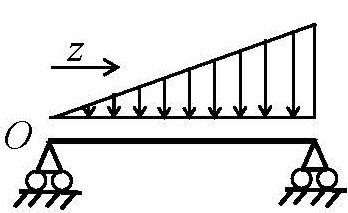
\includegraphics[width=0.15\linewidth]{immagini/1.PARTE2_Pagina_22}
\end{figure}
\[
q(z) = \frac{\tilde{q}z}{l} 
\]
\[
\vec{R} = \int_{0}^{l}\frac{\tilde{q}z}{l}dz = \frac{\tilde{q}}{l} \left[\frac{z^2}{2} \right]_{0}^{l} = \dfrac{\tilde{q}}{l} \frac{l^2}{2} = -\tilde{q} \frac{l}{2} \hat{j}
\]

\[
\vec{M_0} = \int_{0}^{l} z \frac{\tilde{q}}{l} zdz = \frac{\tilde{q}}{l} \int_{0}^{l} z^2dz = \frac{\tilde{q}}{l} \left[\frac{z^3}{3} \right] _{0}^{l} = \frac{\tilde{q}}{l} \frac{l^3}{3} = -\frac{\tilde{q}}{3} l^2 \hat{k}
\]

La posizione della risultante è data dalla media dei carichi pesata con i braccio di ciascuno. 

\[
x_{R} = \frac{\text{forza per braccio}}{\text{risultante}} = \frac{\sum{x_{i}F_{i}}}{R}
\]
\[
z_P = \frac{\int_{0}^{l} z \frac{\tilde{q}}{l} zdz}{\int_{0}^{l}\frac{\tilde{q}z}{l}dz} = \frac{-\frac{\tilde{q}}{3} l^2 }{-\tilde{q} \frac{l}{2}} = \frac{\frac{l}{3}}{\frac{l}{2}} = \frac{2}{3}l
\]

Ci si può così ricondurre ad un problema di carichi concentrati applicati al baricentro del carico distribuito. \newline 

NB: Ricorda che un vincolo esterno non impedisce lo spostamento relativo tra due corpi. \newline

Esempio: \newline 

\begin{figure}[H]
	\centering
	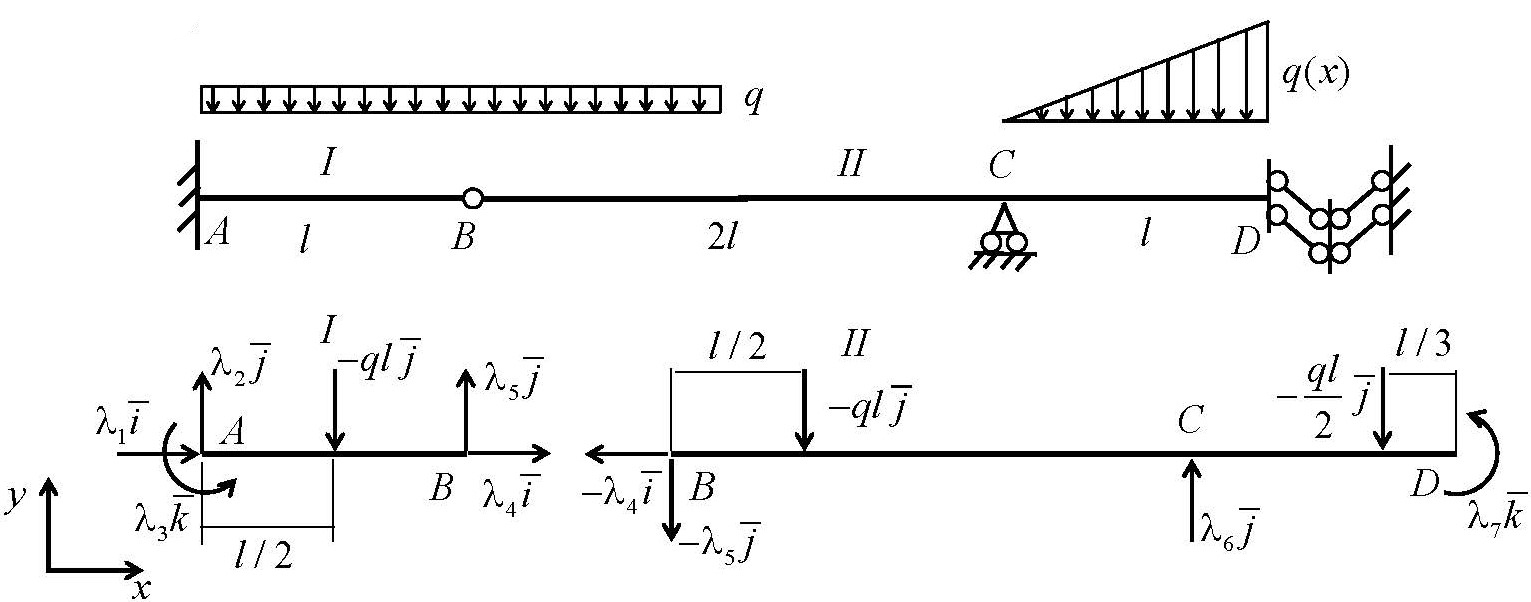
\includegraphics[width=0.4\linewidth]{immagini/1.PARTE2_esempio mancante}
\end{figure} 

Equilibrio del corpo 1:
\[ \begin{cases}
	\begin{aligned}
		R'_x & = \lambda_1 + \lambda_4 = 0 \\
		R'_y & = \lambda_2 - ql + \lambda_5  = 0\\
		M'_A & = \lambda_3 + \left[ \dfrac{l}{2}\hat{i}\times (-ql\hat{j}) + l\hat{i}\times (\lambda_5\hat{j})\right]  = 0 \Rightarrow M'_{Az} = \lambda_3 -\dfrac{ql^2}{2} + l\lambda_5 = 0
	\end{aligned}
\end{cases}\]

Equilibrio del corpo 2: 
\[ \begin{cases}
	\begin{aligned}
		R''_x & = - \lambda_4 = 0 \\
		R''_y & = - \lambda_5 - ql +\lambda_6 - \dfrac{ql}{2} = 0\\
		M''_B & = \lambda_7 + \left[ \dfrac{l}{2}\hat{i}\times (-ql\hat{j}) + 2l\hat{i}\times (\lambda_6\hat{j}) + (2l+\dfrac{2}{3}l)\hat{i}\times (-\dfrac{ql}{2}\hat{j})\right]  = 0 \Rightarrow \\ M''_{Bz} & = \lambda_7 -\dfrac{ql^2}{2} + 2l\lambda_6 - \dfrac{4}{3}ql^2 =0
	\end{aligned}
\end{cases}\]
Un sistema è sempre esprimibile in forma matriciale: 
\[  
\left[ \begin{array}{ccccccc}
	1 & 0 & 0 & 1 & 0 & 0 & 0 \\
	0 & 1 & 0 & 0 & 1 & 0 & 0 \\
	0 & 0 & 1 & 0 & l & 0 & 0 \\
	0 & 0 & 0 & 1 & 0 & 0 & 0 \\
	0 & 0 & 0 & 0 & -1 & 1 & 0 \\
	0 & 0 & 0 & 0 & 0 & 2l & 1
\end{array}\right] \left[ \begin{array}{c}
\lambda_1 \\
\lambda_2 \\
\lambda_3 \\
\lambda_4 \\
\lambda_5 \\
\lambda_6 \\
\lambda_7
\end{array}\right] + \left[ 
\begin{array}{c}
0 \\
-ql \\
-\dfrac{1}{2}ql^2 \\
0 \\
-\dfrac{3}{2}ql \\
-\dfrac{11ql^2}{6}
\end{array}  \right] = 0
\]
In un sistema lineare ci sono tante righe quante equazioni, in questo sistema lineare ci sono 3 equazioni per ogni corpo: 2 corpi portano 6 equazioni. Chiamando "t" il numero di corpi, le righe della matrice sono di numero $3t$. 

In un sistema lineare ci sono tante colonne quante incognite, in questo caso essendoci 7 reazioni vincolari incognite, 7 sarà il numero di colonne della matrice, se a tale numero si da il nome di "s", ci si accorge facilmente che la matrice caratteristica della struttura ha dimensioni:
\[3t\times s\]
Chiamando questa matrice "E", si può infine scrivere: 
\[ [E]_{3t\times s}\vec{\lambda}_s + \vec{f}_{3t} = 0\]

Il sistema si può risolvere ottenendo una soluzione al variare di $\lambda_5 \Rightarrow \exists \infty^1$ soluzioni: 
\[  
\begin{cases}
	\begin{aligned}
		\lambda_4 = 0 \\
		\lambda_1 = 0 \\
		\lambda_5 = k \\
		\lambda_2 = ql - k \\
		\lambda_3 = \dfrac{ql^2}{2} - kl \\
		\lambda_6 = \dfrac{3}{2}ql + k \\
		\lambda_7 = -\dfrac{7}{6}ql -2lk		
	\end{aligned}
\end{cases}
\]
In forma vettoriale:
\[  
\left[ \begin{array}{c}
	\lambda_1 \\
	\lambda_2 \\
	\lambda_3 \\
	\lambda_4 \\
	\lambda_5 \\
	\lambda_6 \\
	\lambda_7
\end{array}\right] = \left[ \begin{array}{c}
0 \\
ql \\
\dfrac{ql^2}{2} \\
0 \\
0 \\
\dfrac{3}{2}ql \\
-\dfrac{7}{6}ql
\end{array}\right] + k \left[ \begin{array}{c}
0 \\
-1 \\
-l \\
0 \\
1\\
1\\
-2l
\end{array}\right]
\]
Le soluzioni di un sistema lineare corrispondono dunque ad una soluzione particolare aggiunta del nucleo della matrice:
\[  \vec{\lambda} = \vec{v} + ker[E]\]
È dunque immediato notare che se:
\begin{itemize}
	\item $ker[E] = 0 \Rightarrow \dim ker[E]=i=0 \Rightarrow i \underset{R_C}{=} s - rk[E] = 0$ la soluzione è unica
	\item $ker[E] \ne 0 \Rightarrow \dim ker[E]=i\ne0 \Rightarrow i \underset{R_C}{=} s - rk[E] \ne 0$ la soluzione è multipla 
\end{itemize}

In questo caso $\dim ker[E]=i=1$: ho bisogno di un parametro variabile per esprimere il nucleo della matrice. \newline

Se la compatibilità descrive le possibilità di trovare l'equilibrio tra forze interne e quelle esterne applicate, la LABILITÀ descriverà la possibilità che ha la struttura di muoversi. \newline
\newpage
{\Large \textbf{Labilità}} \mbox{} \newline		
Si può studiare la possibilità di spostamento di una struttura indipendentemente dai carichi esterni, andando ad analizzare cioè gli spostamenti compatibili con i vincoli: ciò che si vuole fare è in sostanza approfondire la possibilità di movimento della struttura nel piano, analizzare la possibilità che questa ha compiere spostamenti virtuali, in che modo virtualmente la struttura può muoversi nel piano? 

Si noti subito come questo approccio è ben diverso dallo studio dello spostamento causato in seguito all'applicazione di una forza specifica. 
\begin{figure}[H]
	\centering
	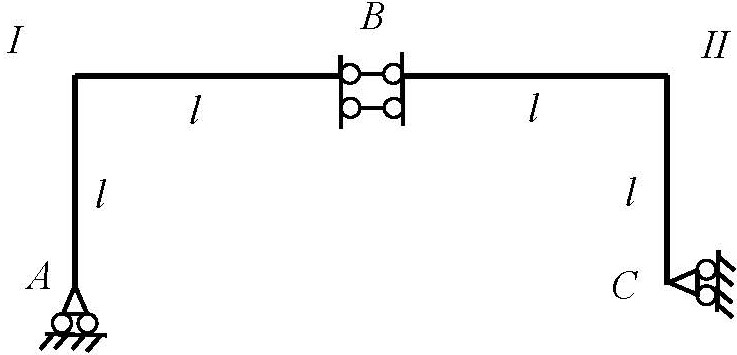
\includegraphics[width=0.4\linewidth]{immagini/1.PARTE2_Pagina_26}
\end{figure}
Quanti vincoli semplici ha la struttura? $s_A = 1 + s_B = 2 + s_C = 1 \Rightarrow s_{TOT} = 4$ ho bisogno di 4 reazioni vincolari per risolvere la struttura. \newline 

Ricordi il concetto di piano mobile? Scelgo ad arbitrio un punto per ogni corpo per descrivere l'intero moto, in questo modo i generici campi di spostamento non terranno conto della presenza dei vincoli, e potranno essere espressi come: 
\[
\vec{s_P}' = \vec{s_A}' + \vec{\Phi}'\times (P-A)
\]
\[
\vec{s_P}'' = \vec{s_B}'' + \vec{\Phi}''\times (P-B)
\]	

Per caratterizzare i possibili spostamenti vincolati vanno conosciuti i descrittori cinematici compatibili coi vincoli, 3 per corpo:
 \[
 s_{Ax}', s_{Ay}', \varphi'_A; s_{Bx}'', s_{By}'', \varphi''_B
 \]

È importante, prima di procedere con lo studio, un'analisi preliminare che permetta di capire se la struttura si muove o meno, solo dopo posso applicare le mie forze fittizie per studiare gli spostamenti che mi interessano. \newline

Devo imporre le restrizioni cinematiche dei vincoli nell'equazione generale precedente. 

\[
A : \text{carrello} \rightarrow \vec{s_A}' \cdot \hat{j} = 0 \Rightarrow 
	\boxed{s_{Ay}'= 0}
\]
Per un vincolo interno ricorda che lo spostamento assoluto può essere qualsiasi, ma quello relativo dev'essere nullo. 
\[
B : \text{d.pendolo} \rightarrow \begin{cases} 
\vec{s_B}'\cdot \hat{i} = \vec{s_B}''\cdot \hat{i} \\
\vec{\Phi}' = \vec{\Phi}''
\end{cases} \Rightarrow \begin{cases} 
s_{Bx}'= s_{Bx}'' \\
\boxed{\varphi'_z = \varphi''_z}
\end{cases}
\]

Sorge a questo punto un problema, se ho scelto per il primo corpo i descrittori cinematici $s'_{Ax}, s'_{Ay},\varphi'_{A}$ dalla prima equazioni del doppio pendolo ottengono un $s_{Bx}'= s_{Bx}''$ in completo disaccordo con la mia scelta, non ho affatto scelto $s_{Bx}'$ per descrivere il primo corpo, quello che devo fare è esprimere questo spostamento in funzione di quelli che ho scelto, e quale relazione usare se non quella universale del generico spostamento con A e B rispettivi poli dei due corpi?
\[ \vec{s}_P = \vec{s}_O + \vec{\varphi} \times (P-O)\]

E allora:
\[
\vec{s_B}'= \vec{s_A}'+ \vec{\Phi}' \times (B-A) = \vec{s_A}' + \varphi_A'\hat{k} \times (l\hat{i} + l\hat{j}) = \vec{s_A}' + \varphi_A'l\hat{j} - \varphi_A'l\hat{i}
\]
Di tutte le componenti presenti mi serve solo quella lungo x:
\[
s_{Bx}'= s_{Ax}'- \varphi_A'l
\]

Infine, sostituendo nell'equazione di partenza $s_{Bx}'= s_{Bx}''$, si ottiene : 

\[
 \boxed{s_{Ax}'- \varphi_A'l = s_{Bx}''}
\]

Anche con carrello si procede come appena visto: non ho scelto il punto C  come descrittore per il corpo II, ma B!
\[
C : \text{carrello} \rightarrow \vec{s_C}'' \cdot \hat{j} = 0 \Rightarrow s_{Cx}'= 0
\]		
Ma:
\[
\vec{s_C}''= \vec{s_B}''+ \vec{\Phi}'' \times (C-B) = \vec{s_B}'' + \varphi''\hat{k} \times (l\hat{i} + l\hat{j}) = \vec{s_B}'' + \varphi''l\hat{j} - \varphi''l\hat{i}
\]
\[
s_{Cx}''= s_{Bx}''+ \varphi''l
\]		
E dunque per i carrello in C si ha: 
\[
\boxed{s_{Cx}''= s_{Bx}''+ \varphi''l = 0}
\]
Si sono trovate in questo modo 4 relazioni che descrivono le restrizioni cinematiche applicate al corpo: 
\[
\boxed{\begin{cases}
	s_{Ay}'= 0 \\
	s_{Ax}'- \varphi'l = s_{Bx}'' \\
	\varphi'_z = \varphi''_z \\
	s_{Bx}''+ \varphi''l = 0
\end{cases}}
\]		
In forma matriciale: 
\[
\left[\begin{array}{cccccc}
	0 & 1 & 0 & 0 & 0 & 0 \\
	1 & 0 & -1 & -1 & 0 & 0 \\
	0 & 0 & 1 & 0 & 0 & -1 \\
	0 & 0 & 0 & 1 & 0 & l
\end{array} \right] \left[ \begin{array}{c}
s_{Ax}' \\
s_{Ay}' \\
\varphi' \\
s_{Bx}'' \\
s_{By}'' \\
\varphi''
\end{array}\right] = \left\lbrace 0 \right\rbrace 
\]	
Si ottiene così una matrice che come numero di righe conta l'esatto numero di vincoli semplici della struttura mentre come numero di colonne ha la quantità $3t$ {\small (dove t è il numero di corpi)} numero dei descrittori cinematici totali. 
\[
[C]_{s\times 3t}\vec{s}_{3t} = [0]
\]		
Nel caso di vincoli ideali.

Con $[C]$ matrice di compatibilità ed $\vec{s}$ vettore degli spostamenti.

Noto che le soluzioni di un sistema lineare omogeneo appartengono al suo nucleo $ker(C)$, allora se: 
\begin{itemize}
\item $\dim\left\lbrace ker(C) \right\rbrace = 0$ l'unica possibilità è lo spostamento nullo, è nulla la possibilità di spostamento della struttura;
\item $\dim\left\lbrace ker(C) \right\rbrace \ne 0$ esistono $\infty^{\dim\left\lbrace ker(C) \right\rbrace }$ spostamenti compatibili con i vincoli.
\end{itemize}		
Si definisce Labilità, caratteristica propria della struttura:
\[
l = \dim\left\lbrace ker(C) \right\rbrace
\]		
Il numero $l$ di parametri indipendenti necessari alla descrizione degli spostamenti virtuali possibili della struttura, si indicano tali spostamenti ammissibili con $\infty^{l}$. \newline

L'analisi statica di una struttura si esegue con $n=3t$ incognite ed $s$ equazioni, in questo modo: 
\[
l = \dim\left\lbrace ker(C) \right\rbrace = 3t - rk(C)
\]		
$[C]$	 è indipendente dai carichi applicati; gli spostamenti considerati nel calcolo della labilità NON sono generati da forze o momenti applicati, sono solo teorici. 

Nell'esempio considerato $rk(C) = 4 \Rightarrow l = 3t - rk(C) = 6-4 = 2 \Rightarrow \infty^2$ spostamenti possibili o possibilità di spostamento. 

Se invece si applicasse un sistema di forze alla struttura, mantenendo la scelta dei poli fatta in precedenza, si otterrebbe: 
\[
E = \left[\begin{array}{cccc}
	0 & 1 & 0 & 0 \\
	1 & 0 & 0 & 0 \\
	0 & -l & 1 & 0 \\
	0 & -1 & 0 & 1 \\
	0 & 0 & 0 & 0 \\
	0 & 0 & -1 & l
\end{array} \right] 
\]	
Che avrebbe condotto anche qua a $\infty^2$ soluzioni. 

Si nota così infine:

\[
C = E^T
\]


\newpage
{\Large \textbf{Vincoli NON Perfetti}} \mbox{} \newline			
Se i vincoli non sono perfetti, questi permettono cedimenti anelastici. 
\begin{figure}[H]
	\centering
	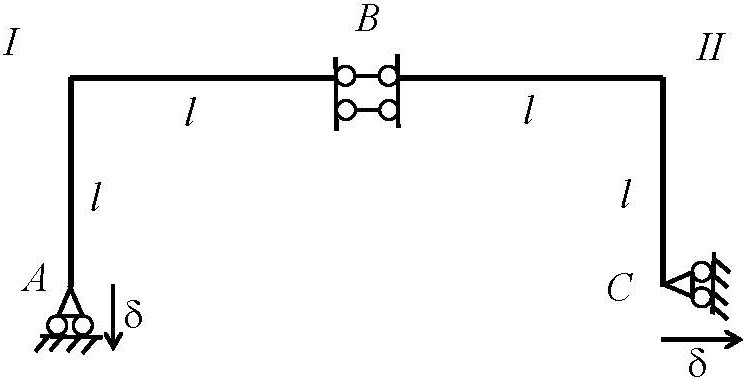
\includegraphics[width=0.15\linewidth]{immagini/1.PARTE2_Pagina_31}
\end{figure}
Nello stesso esempio di prima si pongano con cedimento $\vec{\delta}$ i vincoli $A_{\downarrow}; C_{\rightarrow}$. 

Le limitazioni cinematiche diverranno così: 
\[
\begin{cases}
	s_{Ay}'= -\delta \\
	s_{Bx}' = s_{Bx}'' \\
	\varphi'_z = \varphi''_z \\
	s_{Cx} = \delta
\end{cases}
\]		
In forma matriciale: 
\[
\left[\begin{array}{cccccc}
	0 & 1 & 0 & 0 & 0 & 0 \\
	1 & 0 & -1 & -1 & 0 & 0 \\
	0 & 0 & 1 & 0 & 0 & -1 \\
	0 & 0 & 0 & 1 & 0 & l
\end{array} \right] \left[ \begin{array}{c}
	s_{Ax}' \\
	s_{Ay}' \\
	\varphi' \\
	s_{Bx}'' \\
	s_{By}'' \\
	\varphi''
\end{array}\right] = \left\lbrace \begin{array}{c}
-\delta \\
0 \\
0 \\
\delta
\end{array} \right\rbrace 
\]	

\[
[C]_{s\times 3t}\vec{s}_{3t} =\vec{\delta}_s\]		
Sebbene la matrice $[C]$ non cambi, il sistema NON è più omogeneo. 

La labilità diviene così indice della molteplicità  di una eventuale soluzione, cioè del numero dei parametri rispetto ai quali va scritta la soluzione, non offrendo tuttavia informazioni sull'esistenza delle stesse. 

Per sapere con sicurezza se esiste o meno una soluzione si ricorrerà al teorema di Rouchè - Capelli: c'è possibilità di spostamento? Se e solo se:
\[rk[C] = rk[C\delta]\] 

Vincoli perfetti $\rightarrow$ soluzione $\in$ ker. 

Vincoli non perfetti $\rightarrow$ soluzione $\in$ ker + soluzione particolare. \newline 

Risolvendo col metodo di Gauss si ottiene: 
\[
\left[\begin{array}{cccccc}
	1 & 0 & -l & -1 & 0 & 0 \\
	0 & 1 & -1 & -1 & 0 & 0 \\
	0 & 0 & 1 & 0 & 0 & -1 \\
	0 & 0 & 0 & 1 & 0 & l
\end{array} \right] \left[ \begin{array}{c}
	s_{Ax}' \\
	s_{Ay}' \\
	\varphi' \\
	s_{Bx}'' \\
	s_{By}'' \\
	\varphi''
\end{array}\right] = \left\lbrace \begin{array}{c}
	0 \\
	-\delta \\
	0 \\
	\delta
\end{array} \right\rbrace 
\]	
 E le soluzioni saranno date da: 
 
 \[
 \begin{cases}
x_1 = lx_3 + x_4 \\
x_2 = -\delta \\
x_3 = x_6 \\
x_4 = -lx_6 + \delta \\
x_5 = t_1 \\
x_6 = t_2
 \end{cases} = \begin{cases}
 x_1 = lx_3 -lx_6 + \delta \\
 x_2 = -\delta \\
 x_3 = x_6 \\
 x_4 = -lx_6 + \delta \\
 x_5 = t_1 \\
 x_6 = t_2
\end{cases} = \begin{cases}
s_{Ax}' = x_1 =  \delta \\
s_{Ay}' = x_2 = -\delta \\
\varphi' = x_3 = t_2 \\
s_{Bx}'' = x_4 = -lt_2 + \delta \\
s_{By}'' = x_5 = t_1  \\
\varphi'' = x_6 = t_2 
\end{cases}
 \]
 
 E dunque: 
 \[ 
 \left[ \begin{array}{c}
 	s_{Ax}' \\
 	s_{Ay}' \\
 	\varphi' \\
 	s_{Bx}'' \\
 	s_{By}'' \\
 	\varphi''
 \end{array}\right] = \left[\begin{array}{c}
 \delta \\
 -\delta \\
 0 \\
 \delta \\
 0 \\
 0
\end{array} \right] + \varphi'' \left[\begin{array}{c}
0 \\
0 \\
1 \\
-l \\
0 \\
1 
\end{array} \right] + s_{By}'' \left[\begin{array}{c}
0 \\
0 \\
0 \\
0 \\
1 \\
0 
\end{array} \right] 
\] 

Le soluzioni si ottengono perciò al variare di due parametri. Con il risultato così trovato si può descrivere lo spostamento di qualunque punto del corpo, ma è assai complesso.  \newline

Ho bisogno di uno strumento che mi permetta di visualizzare la mappatura degli spostamenti del corpo dalla lettura di queste matrici.

Da questa scrittura si deve tirar fuori il campo di spostamenti.

Cosa e come si può rappresentare? Attraverso un diagramma si può rappresentare un solo spostamento fisico, virtuale, una configurazione spostata del corpo riconducibile ad un solo set di spostamenti. \newline 

{\Large \textbf{Catene Cinematiche}} \mbox{} \newline		
Cosa si ottiene dalla lettura delle matrici? Le devo tradurre in campi di spostamento. 

Le catene cinematiche sono in grado di rappresentare gli spostamenti di un generico punto P della struttura. 
Si rappresentino gli spostamenti dovuto ai cedimenti della struttura. \newline 

Delle $\infty^l$ soluzioni, ne scelgo di rappresentare una, ad esempio imponendo nelle soluzioni precedenti $\varphi''_A = s''_B = 0$ ottengo: 
 \[ 
\left[ \begin{array}{c}
	s_{Ax}' \\
	s_{Ay}' \\
	\varphi' \\
	s_{Bx}'' \\
	s_{By}'' \\
	\varphi''
\end{array}\right] = \left[\begin{array}{c}
	\delta \\
	-\delta \\
	0 \\
	\delta \\
	0 \\
	0
\end{array} \right] \Rightarrow \begin{cases}
\vec{s_P}' = \vec{s_A}' + \vec{\Phi}'\times (P-A) = \delta\hat{i} - \delta\hat{j} \\
\vec{s_P}'' = \vec{s_B}'' + \vec{\Phi}''\times (P-B) = \delta\hat{i} 
\end{cases}
\] 

In questo modo la chiave della rappresentazione diviene la soluzione della relazione generale degli spostamenti, nella quale sostituisco gli opportuni parametri con i cedimenti. 
\begin{figure}[H]
	\centering
	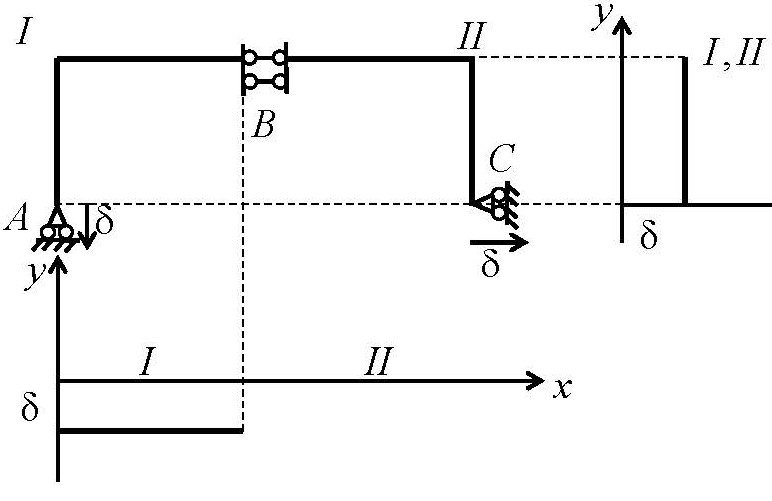
\includegraphics[width=0.3\linewidth]{immagini/1.PARTE2_Pagina_33}
\end{figure}
A destra saranno raffigurati gli spostamenti in direzione x al variare della posizione y, mentre in bassi gli spostamenti in y al variare della posizione x. \newline

Si rappresentino ora gli spostamenti dovuti ai movimenti ammissibili dei vincoli,, si ritorni al caso di vincoli perfetti in cui $s''_B = 0$: 
\[ 
\left[ \begin{array}{c}
	s_{Ax}' \\
	s_{Ay}' \\
	\varphi' \\
	s_{Bx}'' \\
	s_{By}'' \\
	\varphi''
\end{array}\right] = \varphi'' \left[\begin{array}{c}
0 \\
0 \\
1 \\
-l \\
0 \\
1 
\end{array} \right] = t_2 \left[\begin{array}{c}
0 \\
0 \\
1 \\
-l \\
0 \\
1 
\end{array} \right]
\]		
Riscrivo, con queste nuove soluzioni, la mappatura di spostamento: 
\[
\begin{cases}
\vec{s_P}' = \vec{s_A}' + \vec{\Phi}'\times (P-A) = t_1\hat{k} \times (x\hat{i} + y\hat{j}) = t_1x\hat{j} - t_1y\hat{i} \\
\begin{split}
\vec{s_P}'' & = \vec{s_B}'' + \vec{\Phi}''\times (P-B) = -t_1l\hat{i} + t_1\hat{k} \times [(x-l)\hat{i} + (y-l)\hat{j}] = \\
& = -t_1l\hat{i} + t_1(x-l)\hat{j} -  t_1(y-l)\hat{i} = \\
& = t_1y\hat{i} + t_1(x-l)\hat{j}
\end{split}
\end{cases}
\]
Dove i vettori $(P-A), (P-B)$ sono vettori totalmente generici che rispettano i sistemi di riferimenti di ognuno dei corpi. \newline 
		
Per strutture rigide lo spostamento $x$ è tuttalpiù lineare secondo $y$ e lo spostamento $y$ è tuttalpiù lineare secondo $x$.
\begin{figure}[H]
	\centering
	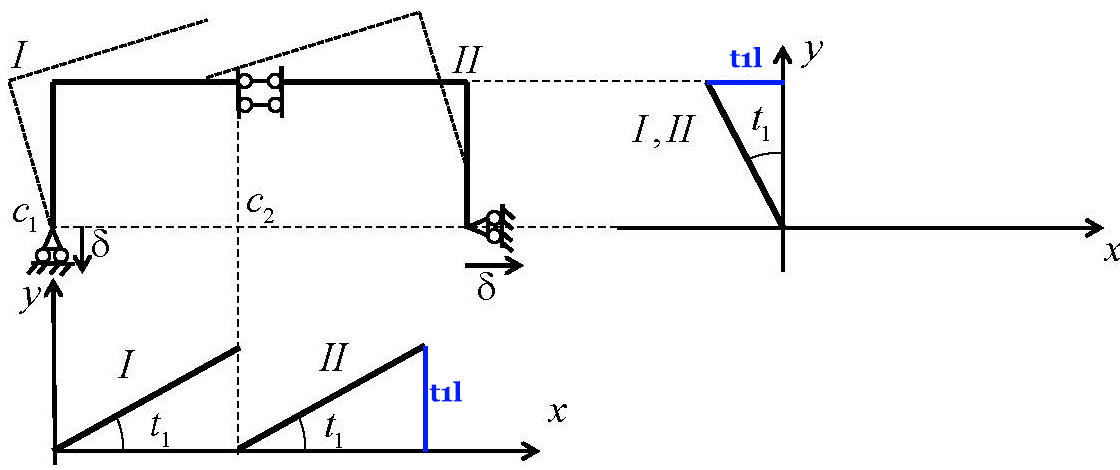
\includegraphics[width=0.3\linewidth]{immagini/1.PARTE2_Pagina_35}
\end{figure}

$t_1$ rappresenta una rotazione infinitesima, cioè un angolo di rotazione della retta che rappresenta in corpo I, lo spostamento sarà dunque $t_1l$. \newline

Le catene cinematiche permettono di rappresentare gli spostamenti di un generico punto della struttura. \newline

Quello che si nota è che si può identificare un punto della struttura caratterizzato da spostamento nullo sia su x che su y, questo punto prende il nome di centro istantaneo di rotazione: è il punto rispetto al quale si può descrivere il moto del corpo come un moto di rotazione pura, è un punto del piano mobile contenente il corpo in esame che ha spostamento nullo. 

NB: non è detto che il punto appartenga al corpo. \newline 

Dunque, se il piano contenente tale punto presenta qualsiasi altro punto a spostamento non nullo, allora lo spostamento di un qualunque punto appartenente la piano mobile considerato può essere rappresentato in funzione di questo centro istantaneo di rotazione. \newline 

Attraverso la catena cinematica si rappresenta così un campo di spostamenti virtuali infinitesimi associati ad un preciso grado di libertà/labilità. 

Quello che si è visualizzato in questo esempio è un campo di spostamenti associato ad un grado di libertà $t_1$, parametro col quale si è indicato l'angolo di rotazione, e degli infiniti valori che può assumere questo parametro, se ne rappresenta uno totalmente arbitrario. \newline 

Con labilità superiore ad uno, si fisseranno valori per ognuna della variabili che si utilizzeranno. 
		
\newpage
{\Large \textbf{Note}} \mbox{} \newline		
		
		
		
		
		
		
%%		\vfill
%\begin{tcolorbox}[height=4.5cm]
%	This box has a height of 1cm.
%\end{tcolorbox}
		
	\end{adjustwidth}
\end{document}